		\newcommand{\OperatorSpaceT}[4]{
				%\draw[rounded corners = 15pt,dashed] (#1-#4,#2-#5) rectangle (#1+#4,#2+#5);
		\fill[fill=green,opacity=0.2] (#1,#2) circle (#3);
		\draw[draw = black,dashed](#1,#2) circle (#3);
		\node at (#1-#3-0.5,#2) {$\region_{#4}$};}
\newcommand{\Vertiports}[4]{
\fill[fill=black,opacity=1.0] (#1,#2) rectangle (#1+0.5,#2+0.5);
\node at (#1+1.0,#2) {$\shield^{#4}_{#3}$};
}

\newcommand{\LoopOver}[5]{
    \path[name intersections={of=#1 and #2}];
            \coordinate (S) at (intersection-1);
            \path[name path=circle] (S) circle(1.0mm);
            \path[name intersections={of = circle and #1}];
            \coordinate (I1) at (intersection-1);
            \coordinate (I2) at (intersection-2);
            \path[draw,very thick] (#3) -- (I1);
            \ifthenelse{#5=1}{\path[draw,very thick,->] (I2) -- (#4);}{\path[draw,very thick] (I2) -- (#4);}
            \tkzDrawArc[color=black,very thick](S,I2)(I1);
}


\definecolor{bodyyel}{HTML}{FFE58F}
\definecolor{bodybl}{HTML}{85A1DC}

    \subfloat[]{\scalebox{0.75}[0.65]{
    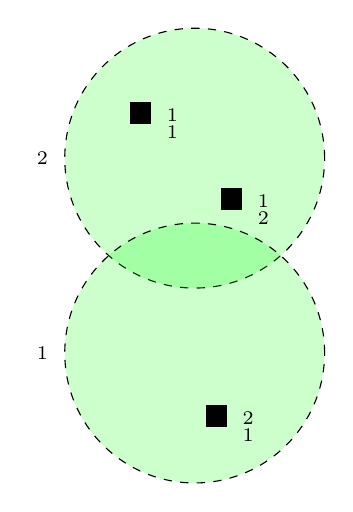
\begin{tikzpicture}[scale=0.55]
			\OperatorSpaceT{0}{0}{3}{2}
			\Vertiports{-1.5}{0.8}{1}{1}
			\Vertiports{0.6}{-1.2}{2}{1}
			\OperatorSpaceT{0}{-4.5}{3}{1}
			\Vertiports{0.25}{-6.2}{1}{2}
			
    \end{tikzpicture}
    }}
\quad
\subfloat[]{\scalebox{0.75}[0.65]{
    \begin{tikzpicture}
            \node[minimum width=1.5cm,rectangle,rounded corners,draw,minimum height=30mm,fill=yellow!20!white] (in) {$\ialphabetx{}$};
            
            
            \node[vert,right=10mm of in.60](vert1){$\shield^1_1$};
            \node[vert,right=10mm of in.40](vert2){$\shield^1_2$};
            \node[vert,right=10mm of in.315](vert3){$\shield^2_1$};
            \coordinate[left=10mm of vert1.205](in1);
            \coordinate[left=10mm of vert2.205](in2);
            \coordinate[left=10mm of vert3.145](in3);
            \coordinate[left=2mm of vert1](v1);
            \coordinate[left=2mm of vert3](v3);
            
            \node[vert,right=20mm of vert1,minimum height=10mm](S1){$S^1$};
            \node[vert,right=20mm of vert3,minimum height=10mm](S2){$S^2$};
            
            \node[hub,right=60mm of vert1] (hub1){$\design_1$};
            \node[hub,right=60mm of vert3] (hub2){$\design_2$};
            

            \path[name path=odest] (in1)--node[above] {} (vert1.205);
            
            \path[->,draw,very thick] (in2)--node[above] {} (vert2.205);
            \path[->,draw,very thick] (in3)--node[above] {} (vert3.145);
            
            \coordinate[right=20mm of vert1.30](c1);
            \coordinate[right=5mm of vert1.330](c2);
            
            % \path[draw,very thick] (vert1.30) |- (c1);
            \path[draw,very thick,->] (vert1.30) -- (c1);
            \path[name path=avail1] (vert1.330) |- (c2);
            % \path[name path=request2,very thick, draw] (vert2.30) -| (c1);
            \path[draw,very thick] (vert2.330) -| (c2);
            
            % \LoopOver{avail1}{request2}{vert1.330}{c2}{0};
            
            
            % \path[->,draw,very thick] (c1) -- node[above]{Ry} (S1.150);
            \path[->,draw,very thick] (c2) -- node[below]{} (S1.210);
            
            \coordinate[above right=10mm and 7.5mm of hub1](out1);
            \coordinate[below right=10mm and 5mm of hub2](out2);
            \path[draw,very thick] (hub1) -| (out1);
            \path[draw,very thick] (hub2) -| (out2);
            \path[->,draw,very thick] (vert3.east) -- (S2.west);
            % \path[->,draw,very thick] (vert3.30) -- node[above]{Rx} (S2.150);
            % \path[->,draw,very thick] (vert3.330) -- node[below]{Ax}  (S2.210);
            

            \coordinate[right=12.5mm of hub1.0] (loiter1);
            \coordinate[right=12.5mm of hub2.0] (loiter2);

            \coordinate[above left=10mm and 5mm of vert1.150] (X1);
            \coordinate[below left=10mm and 5mm of vert3.210] (X2);
            \coordinate[below right=5.5mm and 7.5mm of hub1](Y1);
            \coordinate[above right=6.5mm and 5.0mm of hub2 ](Y2);
            
            \path[->,draw, very thick] (hub1.0) --node[above right]{} (loiter1);
            \path[->,draw, very thick] (hub2.0) --node[above right]{} (loiter2);
            \path[draw, very thick] (out1) -- node[above,name=o1]{$\oalphabetx{1}$} (X1);
            \path[draw, very thick] (out2) -- node[below,name=o2]{$\oalphabetx{2}$} (X2);
            \path[->,draw,very thick](X1) |- (vert1.150);
            \path[->,draw,very thick,name path=land2](X1) |- (vert2.150);
            \path[->,draw,very thick](X2) |- (vert3.210);
            
            \path[draw,very thick] (hub1) -| node[below right] {} (Y1);
            \path[draw,very thick] (hub2) -| node[above right=5mm and 0mm] {} (Y2);
            \path[->,draw,very thick] (Y1) -| (hub2.120);
            \path[->,draw,very thick] (Y2) -| (hub1.280);
            
            \path[->,draw,very thick] (S1) -- node[above]{$\ialphabetx{1}$} (hub1);
            \path[->,draw,very thick] (S2) -- node[above]{$\ialphabetx{2}$} (hub2);
            
            
            \node[fit=(S1)(hub1)(vert1)(vert2)(v1),draw,dashed,minimum width=1.2cm,label={[above]$V^1$}]{};
            \node[fit=(S2)(hub2)(vert3)(v3),draw,dashed,minimum width=1.2cm,label={[below]$V^2$}]{};
            % \node[fit=(S2)(hub2)(vert3),draw,dashed,minimum width=1.2cm,label={[below]$V^2$}]{};
            \node [fit=(in)(o1)(loiter1)(o2),draw,dashed,label={[below right=5.5cm and 6cm of hub2]:{$V$}}] {};
            \LoopOver{odest}{land2}{in1}{vert1.205}{1};
            % \path[name intersections={of=odest and land2}];
            % \coordinate (S2) at (intersection-1);
            % \path[name path=circle2] (S2) circle(1.0mm);
            % \path[name intersections={of = circle2 and odest}];
            % \coordinate (I1) at (intersection-1);
            % \coordinate (I2) at (intersection-2);
            % \path[draw,very thick] (in.45) -- (I1);
            % \path[draw,very thick] (I2) -- (vert1.205);
            % \tkzDrawArc[color=black,very thick](S2,I1)(I2);
		\end{tikzpicture}
		}}
